\documentclass[12pt, a4paper, twoside, openright]{report}
\usepackage[T1]{fontenc}
\usepackage[utf8]{inputenc}
\usepackage[english]{babel}
\renewcommand{\chaptername}{}
\makeatletter
\renewcommand{\@makechapterhead}[1]{%
  \vspace*{50pt}
  {\parindent \z@ \raggedright \normalfont
    \huge\bfseries \thechapter\quad #1\par\nobreak\vskip 40pt}
}
\makeatother
\usepackage[nottoc]{tocbibind}
\usepackage{geometry}
\geometry{
	a4paper,
	left=3cm,
	right=3cm,
	top=3cm,
	bottom=3cm,
	heightrounded
}
% \usepackage{setspace}               % -> Interlinea
% \onehalfspacing
\setcounter{secnumdepth}{2}         % -> Numerazione indice
\setcounter{tocdepth}{3} 
\usepackage{titlesec}
\usepackage{graphicx}               % -> Immagini
\usepackage{tikz}
% \usepackage{subfigure}
\usepackage{float}
% \usepackage{subfigure}
\usepackage{caption}
\usepackage{svg}
% \usepackage{pgfplots}               % -> Plot in latex
% \pgfplotsset{compat=1.18} 
%\usepgfplotslibrary{external}
%\tikzexternalize
\usepackage{listings}
% \usepackage{lipsum}                 % -> Lorem ipsum
\usepackage{afterpage}              % -> Blank numbered page
% \usepackage{newtxtext,newtxmath}    % -> Times new romans
\usepackage{enumerate}
\usepackage[RPvoltages]{circuitikz} % -> Schematic design
\usepackage{xcolor}                 % -> Colori
\usepackage{fancyvrb}               % -> codice colorato in verbatim
\usepackage{pdfpages}               % -> Inserisce pdf 
\usepackage{subfiles}
\usepackage[toc,page]{appendix}     % -> Appendix
\addto\captionsitalian{%
   \renewcommand{\appendixtocname}{Appendici}%
   \renewcommand{\appendixpagename}{Appendici}%
}

\usepackage{amsfonts}               % -> Math
\usepackage{amsmath}
\usepackage{xfrac}                  % -> sfrac
\usepackage{rsfso}                  % -> Font for the Laplace L
\usepackage{booktabs}               % -> Tabelle
\usepackage{makecell}
\usepackage{multirow}
\usepackage{siunitx}                % -> Rappresentzione dei numeri migliore (SI) 
                                    %    (https://texdoc.org/serve/siunitx/0)
                                    
\usepackage[hidelinks]{hyperref}    % -> Hyperlink
% \hypersetup{
%     colorlinks=true,
%     linkcolor=black,
%     filecolor=magenta, 
%     urlcolor=blue,
%     pdfborder={1 0 0},
%     linkbordercolor=red,
% }

\hypersetup{
    colorlinks,
    linkcolor={black!100!black},
    citecolor={black!100!black},
    urlcolor={black!100!black}
}

% Line above footer and below header
\usepackage{fancyhdr} 

\usepackage{pdfpages} % Per includere più pagine di PDF

\usepackage[absolute,overlay]{textpos}

\pagestyle{fancy}   % Change page style to fancy
\fancyhf{}  % Clear all header and footer fields
\fancyhead[LE]{\leftmark}
\fancyhead[RO]{\rightmark}
\fancyfoot[CO, CE]{\thepage}
\renewcommand{\headrulewidth}{0.4pt} % Default \headrulewidth is 0.4pt
\renewcommand{\footrulewidth}{0.4pt} % Default \footrulewidth is 0pt
\setlength{\headheight}{15pt}

% Roman number
\makeatletter
\newcommand*{\rom}[1]{\expandafter\@slowromancap\romannumeral #1@}
\makeatother

% completely blank page
\newcommand\blankpage{%
    \null
    \thispagestyle{empty}%
    \addtocounter{page}{-1}%
    \newpage
}

\title{EcoTraffic}
\author{Lorenzo Esposito, Alessandro Frisone, Francesco Grassi, Giorgio Venezia}
\date{\today}


\begin{document}

\begin{textblock*}{\textwidth}(2.98cm,1.5cm)
  \begin{center}
    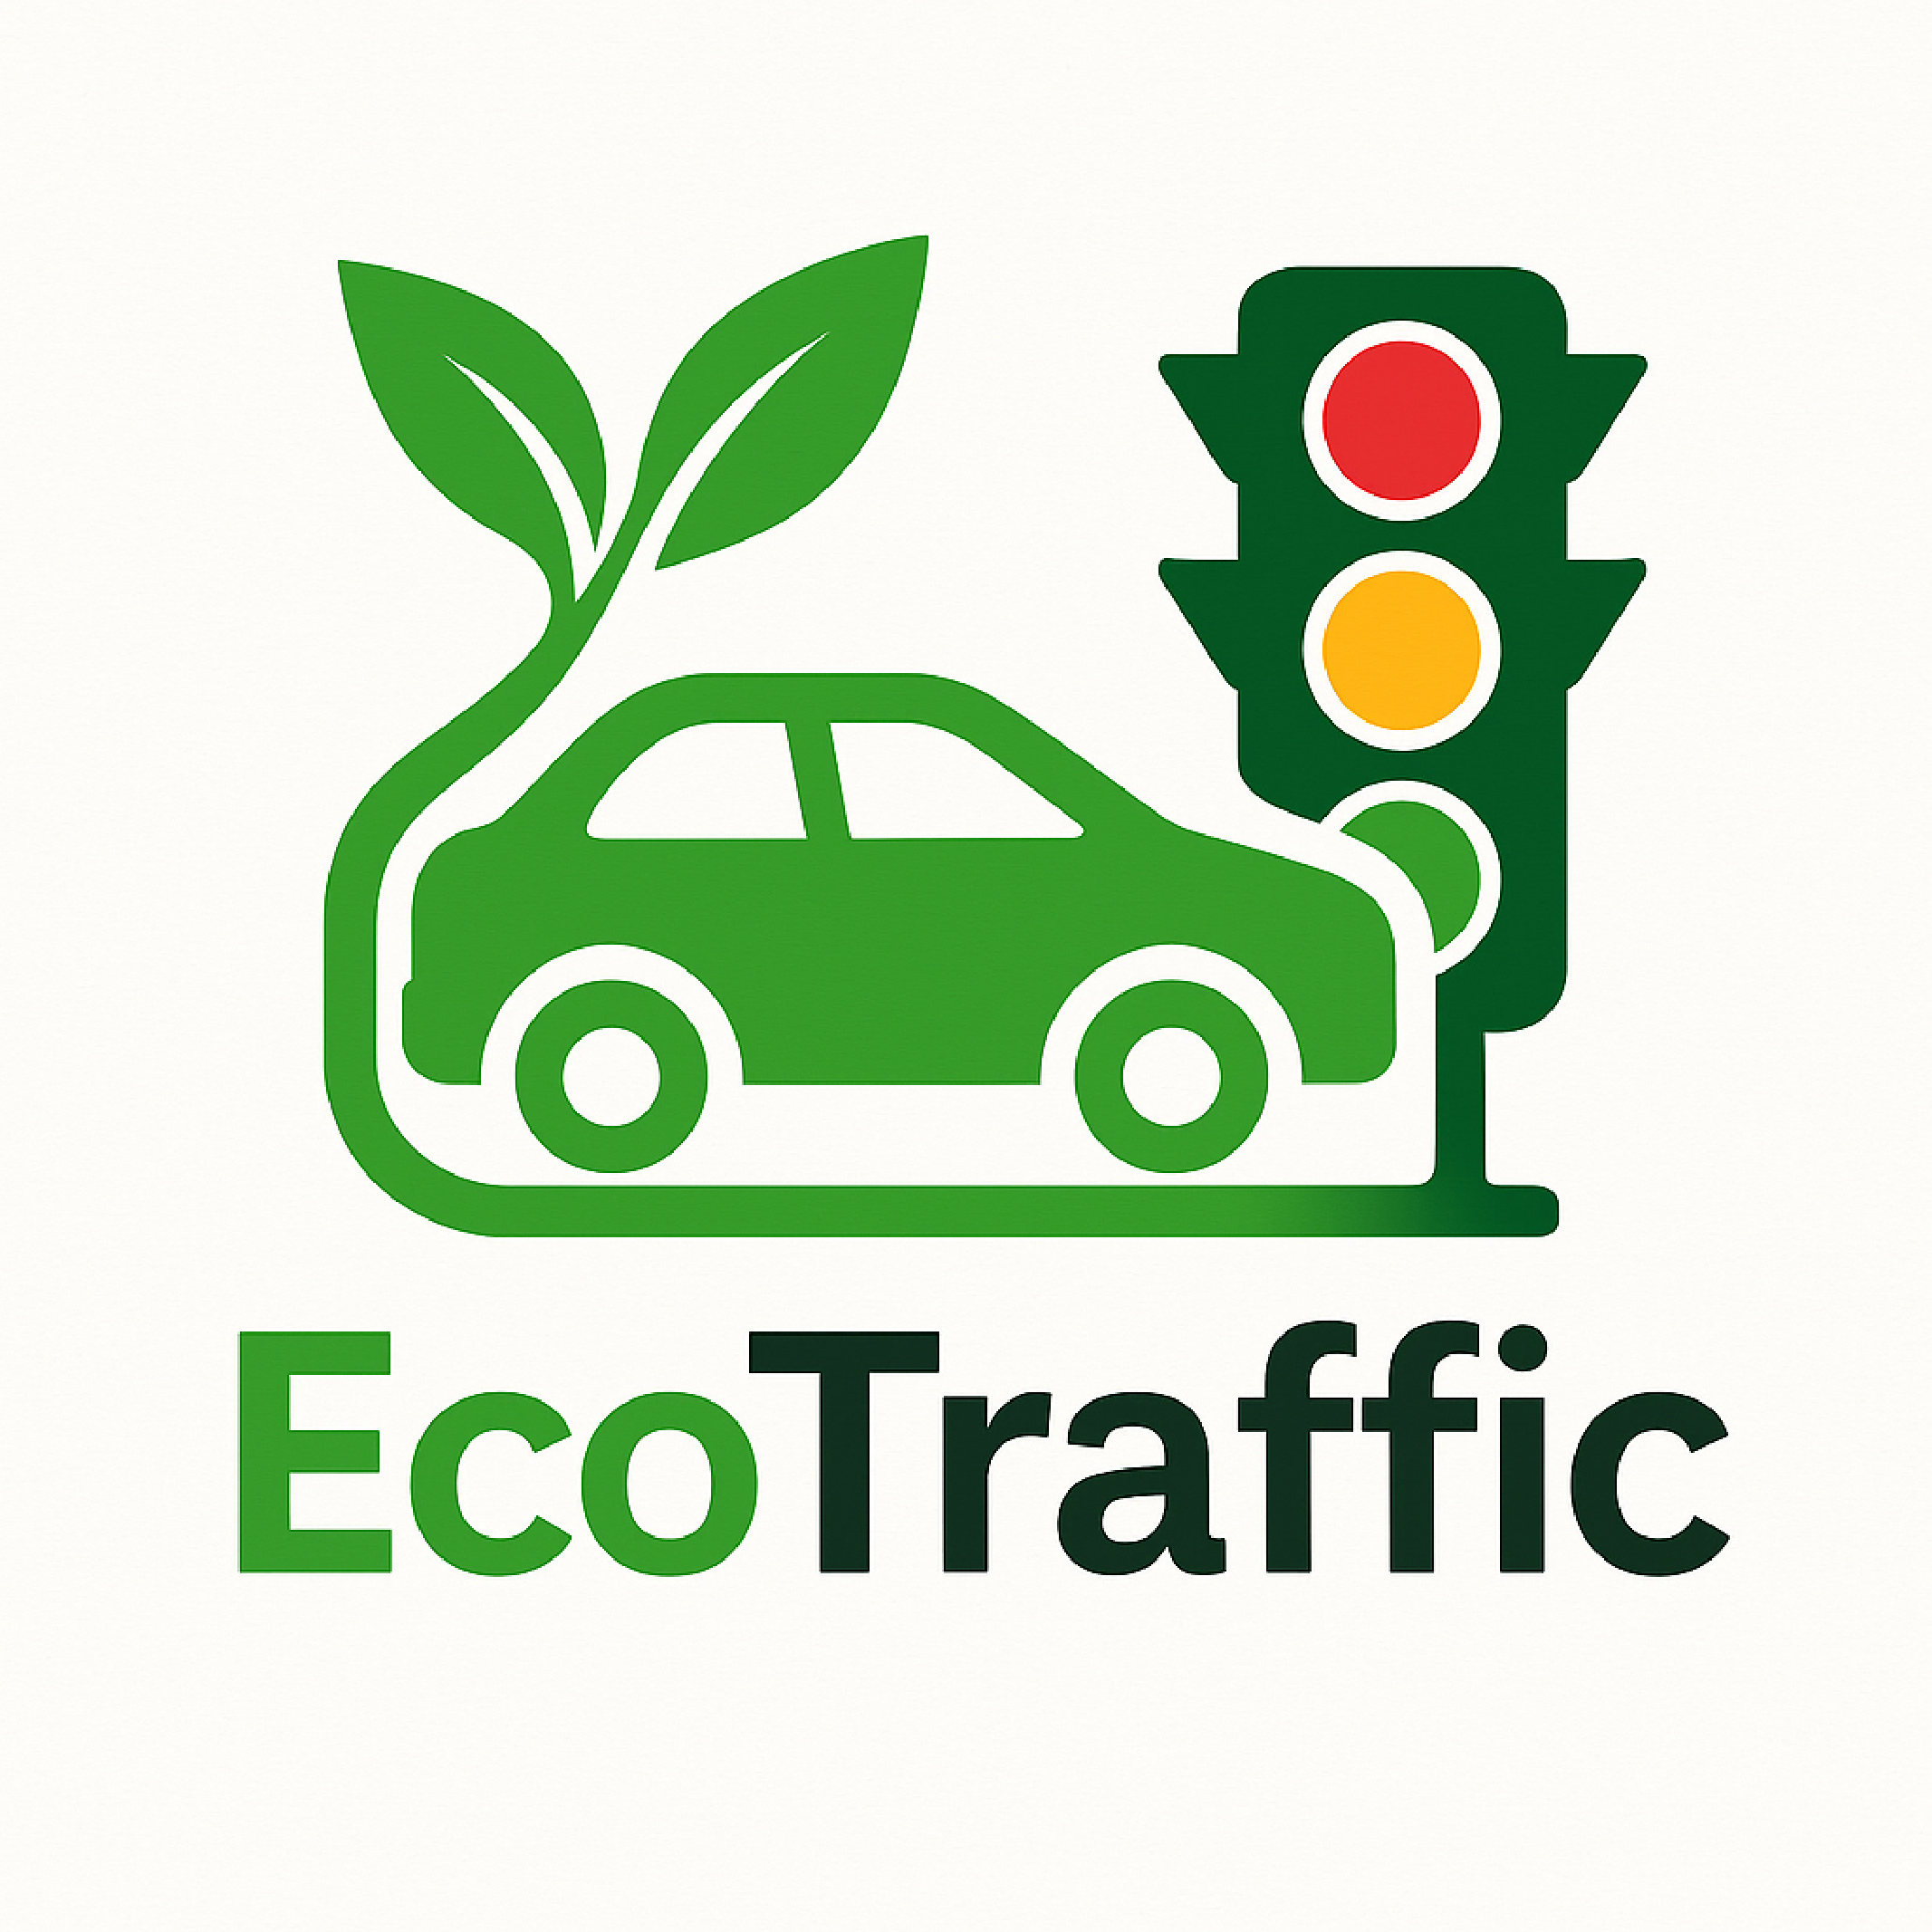
\includegraphics[scale=0.25]{images/EcoTraffic_logo.pdf}  
    \maketitle
    Version 1.0.0
  \end{center}  
\end{textblock*}


\blankpage

% ============== Indice ============== %
\pagenumbering{roman}
\tableofcontents
\afterpage{\blankpage}
\newpage
\pagenumbering{arabic}

\chapter{The Project and the project goals}
\section{The problem}
Two urgent global concerns are environmental sustainability and climate
change; because of air pollution and greenhouse gas emissions,
transportation, especially urban commuting, contributes to worsening
those issues.
\section{The goal}

We want to dynamically modify the duration of traffic lights on the main
roads in the city depending on the directions from where we observe the
main traffic movements. For instance, if, at a certain point in time, we
observe that the traffic flow on a certain road A is significantly
higher than in the crossing roads, then we may decide to extend, for
instance, for one hour, the duration of green lights on A (and,
consequently, extend the duration of red lights in the crossing
roads).\\
We want to analyze the daily traffic patterns and identify possible
optimizations in terms of one-way roads, traffic lights configuration,
and public transport schedule.\\
We want to collect information about the planning of events attracting
large crowds (e.g., important sport events, concerts, fairs) and define
event-specific configurations for traffic lights, roads and public
transport schedules.

\section{Stakeholders}

  \begin{itemize}
    \item Drivers: for reduced waiting times stuck in the traffic.
    \item Citizen: for air pollution, public transport.
    \item Urban Area manager: for optimization of city viability.
    \item Events planner: for a better management of events attracting large crowds.
  \end{itemize}

\chapter{Requirement Analysis}
\section{Relevant human and non-human actors}
\subsection{Human Actors}
\begin{itemize}
  \item Drivers: benefit from the EcoTraffic system.
  \item Citizen: benefit from the EcoTraffic system.
  \item Urban Area manager: approve or rejects modifications to one-way roads, traffic lights configuration, and public transport schedule.
\end{itemize}

\subsection{Non-Human Actors}
\begin{itemize}
  \item Traffic Lights: get its state set from the ET system for a determined time period.
  \item Sensor Infrastructure: send sensor information to the ET system via data bus.
  \item Public Transport Microservice: sends public transport schedules to the EcoTraffic system via function calls.
  \item News Channel: transmits city events information to the ET system.
\end{itemize}

\section{Use Cases}\label{sec:use-cases}
\subsection{Scenarios (to modify)}\label{subsec:scenarios}

\subsubsection{Traffic light duration adjustment}\label{subsubsec:traffic-light-duration}

\begin{enumerate}
\item
  During peak traffic hour, cars take more than the necessary to cross a
  particular intersection coming from a busy road, while the crossing
  road are less used.
\item
  The system sensor measures the times taken and publish them on the
  data bus.
\item
  EcoTraffic retrieves the data from the data bus and stores them into a
  database.
\item
  EcoTraffic tries to catch misbehaviour.
\item
  If a misbehaviour is detected, then EcoTraffic compute the new
  routines time for the traffic light which must be modified.
\item
  EcoTraffic connects to the traffic light control system providing
  serial numbers of the traffic lights which must modify the routine
  with the amount of time interval to be changed.
\item
  EcoTraffic writes into a log file the modifications done.
\end{enumerate}

\subsubsection{Daily Analysis and optimization}\label{subsubsec:daily-analysis}

\begin{enumerate}
\item
  Ten minutes after midnight, EcoTraffic retrieve daily data from the
  database.
\item
  EcoTraffic analyse this data to detect daily traffic pattern and to
  find possible optimization in term of one-way roads, traffic lights
  configuration, and public transport schedule.
\item
  EcoTraffic performs the getScheduleByStreet and the getScheduleByLine
  offered by the microservice.
\item
  EcoTraffic tries to reorganize the schedules to optimize the public
  transport.
\item
  If possible optimizations are found, EcoTraffic store them into the
  database.
\item
  Once the UAM access the system, it presents the optimizations found
  and wait for the answer of the UAM.
\item
  EcoTraffic writes into a log file the answer for yearly reporting.
\end{enumerate}

\subsubsection{Traffic Zone Optimization}\label{subsubsec:traffic-zone}

\begin{enumerate}
\item
  The Urban Area Manger asks to EcoTraffic to verify if a certain zone
  is optimized in terms of one-way roads, traffic lights configuration,
  and public transport schedule.
\item
  EcoTraffic retrieve from the database the traffic patterns of the
  zone.
\item
  EcoTraffic analyses the data retrieved and tries to minimize the
  medium amount of time taken to cross an intersection into the zone.
\item
  EcoTraffic performs the getScheduleByStreet and the getScheduleByLine
  offered by the microservice to get all the bus lines that has a stop
  into the area to optimize.
\item
  After the information arrived, EcoTraffic tries to reschedule the
  timetable of the bus lines in such a way to minimize the traffic. (i.e
  if in the zone there's a school, then the system could anticipate the
  timetable of the stops near that to avoid the students to arrive late
  or could suggest increasing the number of buses in the area).
\item
  EcoTraffic presents to the UAM the recommendations and waits till the
  UAM decide to accept or to reject the recommendation and store the
  decision.
\item
  EcoTraffic writes into a log file the answer for yearly reporting.
\end{enumerate}

\subsubsection{Event-specific configurations}\label{subsubsec:event-specific}

\begin{enumerate}
\item
  News channel publishes information about upcoming event with the
  expected attendance.
\item
  EcoTraffic receives the event information via integration with news
  channel.
\item
  EcoTraffic automatically categorizes the event by the attendance.
\item
  EcoTraffic analyzes historical traffic patterns from similar events.
\item
  EcoTraffic retrieves public transport schedules via microservice using
  getScheduleByStreet and getScheduleByLine operations.
\item
  EcoTraffic generates event-specific configuration recommendations for
  traffic lights and roads.
\item
  The UAM accesses to EcoTraffic and reviews the suggestions proposed
  and decides to accept or to reject them.
\item
  EcoTraffic writes into a log file the answer for yearly reporting.
\end{enumerate}

\subsubsection{System monitors traffic during special event (forse da togliere,
altrimenti si deve modificare l'architettura)}\label{subsubsec:system-monitors}

\begin{enumerate}
\item
  EcoTraffic detect the presence of a special event happening today.
\item
  Traffic sensors detect traffic flow.
\item
  Traffic sensors publish data to message bus.
\item
  EcoTraffic receives sensor data from message bus.
\item
  EcoTraffic retrieve the data in the area near the event.
\item
  EcoTraffic implements temporary traffic light timing changes if
  needed.
\item
  EcoTraffic logs all adjustments and their effectiveness
\item
  EcoTraffic updates event-specific configuration data based on
  observations for future similar events
\end{enumerate}

\subsubsection{Citizen views public traffic reports}\label{subsubsec:citizen-views}

\begin{enumerate}
\item
  Citizen accesses EcoTraffic public portal.
\item
  EcoTraffic presents options for viewing reports.
\item
  Citizen selects the preferred option.

  \begin{enumerate}
  \item
    Citizen selects "Daily Traffic Reports" and choose the date and
    time.
    \begin{enumerate}
    \item
      EcoTraffic retrieves daily report data from database service.
    \item
      EcoTraffic displays report showing:

  \begin{enumerate}
        \def\labelenumiv{\alph{enumiv}.}
        \item
          Average traffic flow on main roads.
        \item
          Visualization of peak congestion periods.
        \item
          List of actions taken automatically.
        \item
          Traffic prediction for tomorrow.
        \end{enumerate}
      \end{enumerate}
    \item
      Citizen selects "Yearly Reports" option.
  
      \begin{enumerate}
      \item
        EcoTraffic displays yearly report options.
      \item
        EcoTraffic retrieves yearly report data from database service.
      \item
        EcoTraffic displays comprehensive report showing:
  
        \begin{enumerate}
        \def\labelenumiv{\roman{enumiv}}
        \item
          Suggested actions that were accepted.
        \item
          Suggested actions that were rejected.
        \end{enumerate}
      \end{enumerate}
    \end{enumerate}
  \end{enumerate}

\subsubsection{UAM views optimization to approve or reject}\label{subsubsec:uam-views}

\begin{enumerate}
\item
  UAM access to EcoTraffic public portal.
\item
  EcoTraffic displays all the suggested changes not already approved or
  rejected.
\item
  The UAM analyse each suggestion and decide to approve or reject
  choosing an option displayed.
\item
  EcoTraffic writes into a log file the answer for yearly reporting.
\end{enumerate}

\subsection{Use case diagrams (to modify)}
\subsubsection{Traffic light duration adjustment}
Actors: Sensors, Traffic lights, database.

Entry condition: After sensors measures new crossing times, new data
arrives on the bus.

Flow of events:

\begin{itemize}
\item
  EcoTraffic reads data from the message bus.
\item
  EcoTraffic stores in the database the data received.
\item
  EcoTraffic compares the crossing times of the roads in the crossings.
\item
  If EcoTraffic detects traffic load imbalance, the system computes the
  green light duration to optimize vehicle flow in the more congested
  direction.
\end{itemize}

Exit condition: The system sends the adjusted times to the traffics
lights control system.


\subsubsection{Daily Analysis and Optimization}
Actors: Webservice, database

Entry condition: It's ten past midnight.

Flow of events:

\begin{itemize}
\item
  EcoTraffic queries the database to get all the crossing times measured
  in the day before.
\item
  EcoTraffic analyses the data retrieved to obtain traffic pattern.
\item
  EcoTraffic analyses the traffic pattern to find possible optimization
  in terms of one-way roads and traffic lights configuration.
\item
  EcoTraffic retrieves public transport schedules via microservice using
  getScheduleByStreet and getScheduleByLine operations.
\item
  EcoTraffic tries to find better schedules for the public transport
  line.
\end{itemize}

Exit condition: The system write into the database the possible
optimization found.


\subsubsection{Traffic zone optimization}

Actors: Urban area manager, Public Transport Microservice, database

Entry condition: UAM accesses EcoTraffic public portal and decide to
request optimization of a certain area.

Flow of events:

\begin{itemize}
\item
  EcoTraffic queries the database to obtain the crossing times of the
  zone indicated by the UAM
\item
  EcoTraffic analyses the data to find possible optimization in terms of
  one-way roads and traffic lights configuration.
\item
  EcoTraffic retrieves public transport schedules via microservice using
  getScheduleByStreet and getScheduleByLine operations.
\item
  EcoTraffic tries to find better schedules for the public transport
  line.
\item
  The system sends the new scheduling and configurations proposal to the
  UAM for approval.
\item
  The system waits for the answer.
\item
  When the decision is taken, the answer is written into a log file.
\end{itemize}

Exit condition: Successful write of the log.


\subsubsection{Event-specific configurations}


Actors: News channel, UAM, Public transport microservice

Entry condition: News channel publishes information about upcoming
events.

Flow of events:

\begin{itemize}
\item
  EcoTraffic categorizes the scale of the event by attendance.
\item
  EcoTraffic investigates the database for historical traffic patterns
  and past decision tskrn in similar events in previous log files.
\item
  EcoTraffic retrieves public transport schedules via microservice using
  getScheduleByStreet and getScheduleByLine operations.
\item
  Using the collected data, EcoTraffic generates event-specific
  configurations that are optimized in terms of one-way roads, traffic
  lights configuration and public transport schedules.
\end{itemize}

Exit condition: The system write into the database the possible
optimization found.


\subsubsection{System monitors traffic during special event}


Actors: Sensors, traffic lights, Public transport microservice

Entry condition: EcoTraffic detects an event on that specifi day from
the News channel.

Flow of events:

\begin{itemize}
\item
  The system looks for historical traffic patterns in the area and at
  the time before/during/after the event.
\item
  The system retrieves public transport schedule via microservice.
\item
  The system periodically collects data from the bus. todo
\item
  The system periodically compute an optimization for the traffic lights
  on the roads impacted by the event using the collected data.
\item
  The system updates event-specific configuration data based on
  observations for future similar events.
\item
  The system logs all adjustments and their effectiveness.
\end{itemize}

Exit condition: Successful write of the log.

\subsubsection{Citizen views public traffic reports}


Actors: Citizen

Entry condition: Citizen accesses EcoTraffic public portal.

Flow of events:

\begin{itemize}
\item
  The system presents options for viewing reports.
\item
  The citizen selects the type of information that they want to be
  displayed.
  
\item 
  The system retrieves daily or yearly data from database service.
\item  
  The system elaborates the data to facilitate interpretation.  
\item  
  The system displays a report with the elaborated data.  
\item  
  The citizen chooses between seeing more information or exiting the
  portal.  
\end{itemize}

Exit condition: The citizen exits the portal.


\subsubsection{UAM views optimization to approve or reject}

Actors: UAM

Entry condition: UAM accesses EcoTraffic public portal and decide to
view the optimization waiting for approval.

Flow of events:

\begin{itemize}
\item
  
  EcoTraffic queries the database for the optimization proposals waiting
  for approval.
  
\item
  
  EcoTraffic elaborates the data to facilitate interpretation.
  
\item
  
  EcoTraffic displays all the decision to be taken.
  
\item  
  EcoTraffic waits for the UAM to answer to each request.
  
\item
  
  Every time a decision is taken EcoTraffic stores it into a log file.
  
\end{itemize}

Exit condition: All the decision have been taken.

\section{Domain assumption}
\begin{enumerate}
\item
  The sensor infrastructure works correctly and with low latency 24/7.
\item
  The traffic lights are not faulty and set their state correctly in
  time from the ET system.
\item
  Drivers behave accordingly to the traffic light state.
\item
  No car can obstruct the passage in the crossing no matter the reason.
\item
  Events planners always report to the news channel up to date events in
  the city.
\item
  The public Transport Microservice always returns the right timetable
  given a line or the name of a street.
\end{enumerate}
\section{Requirements}
\subsection{Functional Requirements (to modify put id of each
  requirement. Es FR1\ldots)}

\begin{enumerate}
\item
  In any circumstance the system must not allow two orthogonal traffic
  lights to be green at the same time.
\item
  The system must modify the duration of the green lights to reduce
  traffic.
\item
  The system shall process and aggregate traffic data to identify
  traffic flow patterns.
\item
  The system should send adjustment commands to the traffic light
  control system.
\item
  The system should be able to write to a log file what needed.
\item
  The system shall generate optimization suggestions for one-way road
  and traffic light configurations.
\item
  The system shall generate optimization suggestions for public
  transport schedules.
\item
  The system shall continuously receive data from both the message bus
  and the news channel.
\item
  The system must gather data from the microservice.
\item
  The system must assess the potential traffic impact of planned events.
\item
  The system shall generate event-specific suggestions for public
  transport adjustments.
\item
  The system shall present suggestions to urban area managers for
  review.
\item
  The system shall record and apply the acceptance or rejection of the
  proposal by the urban area managers.
\item
  The system shall generate daily reports on average traffic flow.
\item
  The system shall generate yearly reports on suggestions proposed and
  their outcome.
\item
  The system shall publish reports for public access.
\end{enumerate}

\subsection{Non-Functional Requirements}

\begin{enumerate}
\item
  The system shall process sensor data in real time.
\item
  The system should be available 24/7.
\item
  The system shall implement traffic light adjustments in 15 seconds.
\item
  The system shall generate reports within 1 hour after midnight.
\item
  The system should maintain data consistency during communication with
  external systems.
\item
  The system should be scalable regarding the addition of sensors and
  bus lines.
\end{enumerate}

\subsection{Constraints (to modify, insert something to use the
external services)}

\begin{enumerate}
\item
  The setLight function must be atomical.
\item
  The call to the microservice must be done using an API REST.
\end{enumerate}

\chapter{Design}

\section{Architecture}
\subsection{Components diagram}

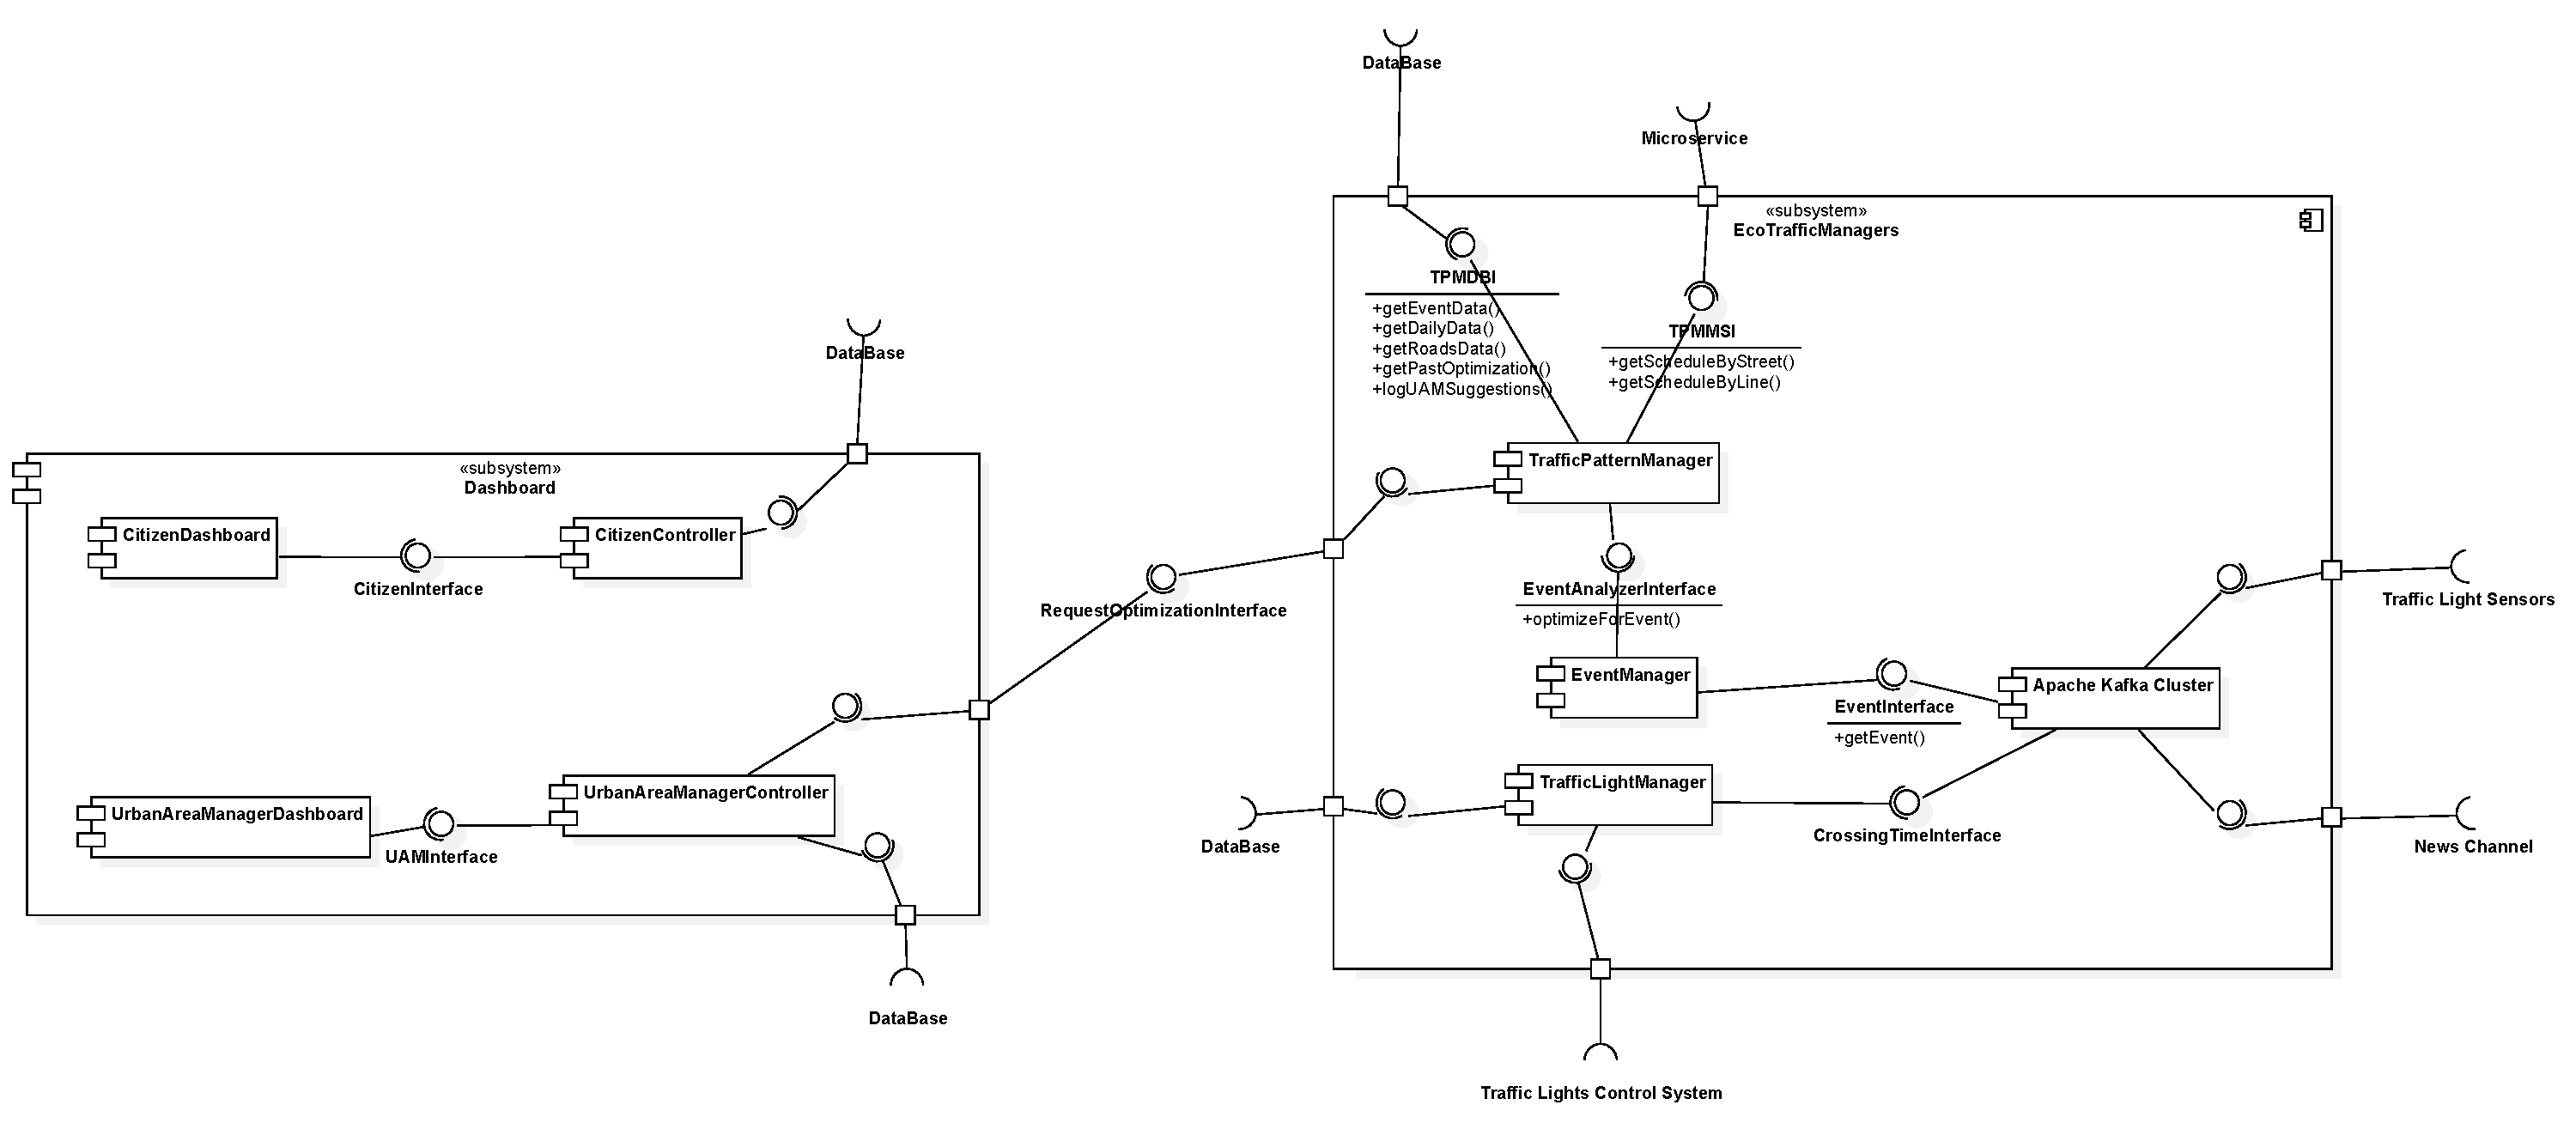
\includegraphics[width=\linewidth]{images/svg/component_diagram.pdf}
In this diagram, we've insert multiple interface called "database" for readibility, actually there's only database which
structure is shown in the next diagram.\\
\subsection{Subsystems and components}

The EcoTrafficManagers subsystem includes the component:


\begin{itemize}
\item
  \textbf{ApacheKafkaCluster:} the component is based on a framework for
  event-driven paradigm and it includes primitives to create event
  producers and consumers and a runtime infrastructure to handle event
  transfer. This component it's the one responsible to receive the data
  from the sensors system and from the news channel and to distribute
  them to the right components who then will process and analyse them.
  More information could be found at \url{https://kafka.apache.org/}.
\item
  \textbf{TrafficLightManager:} this component receives the data
  measured by the sensors system from the ApacheKafkaCluster and
  provides method to analyse this data to find unbalanced traffic loads
  into a crossing, to compute the new time in which the green light is
  switched on to reducing traffic congestion, to store into the database
  of the system the data obtained from the ApacheKafkaCluster and to
  connect to the control system of the traffic lights to apply the right
  modifications.
\item
  \textbf{EventManager:} this component receives the event specification
  from the ApacheKafkaCluster after that the news channel has published
  them. This component provides methods to retrieve information (such
  that the event type, the date, the place and the expected attendance)
  and a method to call the TrafficPatternManager component to optimize
  the event configuration to reduce traffic load.
\item
  \textbf{TrafficPatternManager:} this component could be called by
  three events. The first is when the EventManager calls it to perform
  event-based optimization, in this case the component queries the
  database to find similar event and the daily traffic patterns in the
  zone where the event takes place, then generate possible optimizations
  from this data and from the timetables obtained after the
  getScheduleByStreet() and the getScheduleByLine() calls to the
  microservice. The second is when the UrbanAreaManagerController asks
  for an optimization around a specific zone, in this case the component
  queries the daily traffic patterns in the zone and the timetables and
  tries to optimize the traffic loads. The third takes place
  automatically ten minutes after the midnight, in this case the
  component queries the daily crossing time in all the crossings of the
  area and finds traffic patterns, after that it tries to optimize in
  terms of one-way roads, traffic lights configuration, and public
  transport schedule.
\end{itemize}

The Dashboard subsystem includes the following components:

\begin{itemize}
\item
  \textbf{CitizenDashboard:} this component shows to the citizen an
  interface from where it can be decided to see the daily reports or the
  yearly one. After choosing, the component calls the CitizenController
  to get the reports. When the response arrives, the component shows to
  the user the reports.
\item
  \textbf{CitizenController:} this component receives the request from
  the citizen dashboard and them queries the database to satisfy the
  request. After, the data are elaborated and sent to the dashboard.
\item
  \textbf{UrbanAreaManagerDashboard:} this component shows to the UAM an
  interface from where it can be decided if to see the pending
  suggestions or to ask the system to optimize all the configurations in
  a precise zone. If the first option is taken, the calls the
  UrbanAreaManagerController to get the pending suggestions. When the
  response arrives, the component shows to the user the reports and
  waits till all the decisions are taken. When each decision is taken,
  the component sends the answer to the controller. If the second option
  is taken, the dashboard presents the zones in the area and waits for
  the UAM's decision, after it arrives the components sends to the
  controller the requests and waits for the answer, after this arrives
  it displays to the UAM the suggestions, when the decision is taken,
  the component sends the answer to the controller.
\item
  \textbf{UrbanAreaManagerController:} this component is responsible for
  managing the requests arriving from the dashboard and to redirect them
  either to the database if the UAM wants to see the pending suggestions
  or to the TrafficPatternManager if the UAM wants an optimization for a
  specific zone. After the responses arrive, the component sends them to
  the dashboard. If the answer it's an optimization the component waits
  for the approval or the rejection and stores the decision.
\end{itemize}
  
\section{Sequence Diagrams}
\subsubsection{Traffic Lights Adjustment}

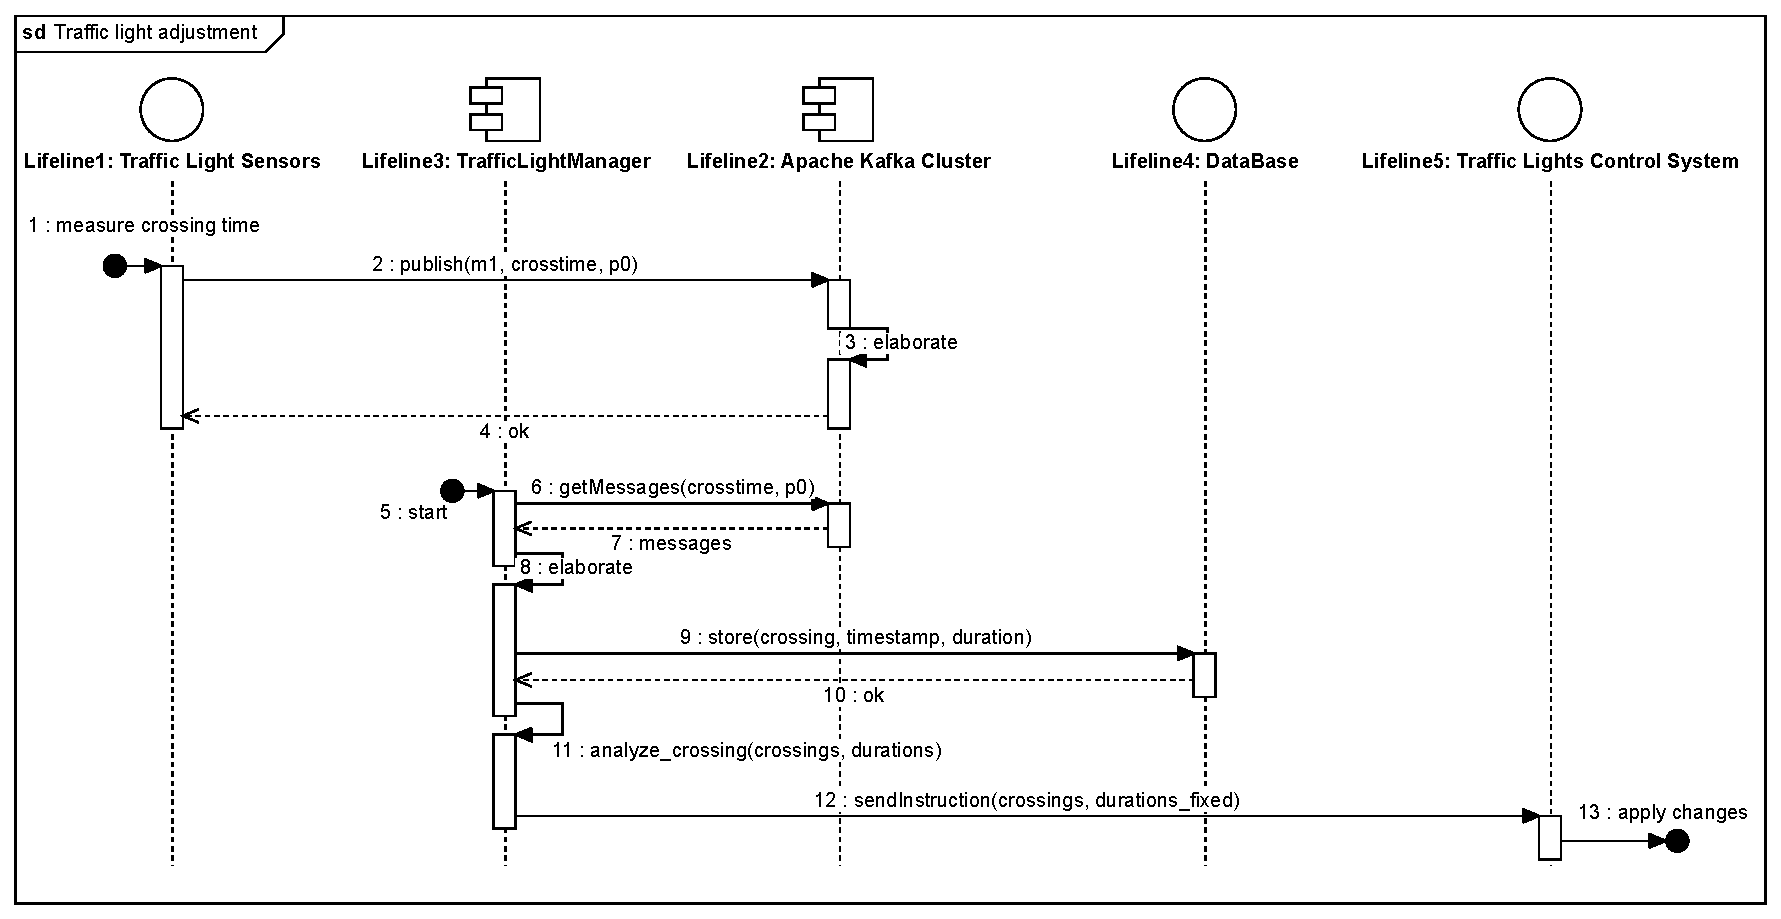
\includegraphics[width=\linewidth]{images/svg/traffic_light_adjustment.pdf}

This sequence diagram shows the communication and data flow involved in
adjusting traffic light timings based on crossing data.

\begin{enumerate}
\item
  The traffic light sensors system measures a crossing time.
\item
  The traffic light sensors system publishes the crossing time on the
  message bus and it's received from the Apache Kafa Cluster.
\item
  The Apache Kafka Cluster performs the operation as shown in this
  diagram.
\item
  The AKC responds to the traffic light sensors system.
\item
  TrafficLightManager is working.
\item
  TrafficLightManager tries to get a message.
\item
  The message, if present, it's sent to TrafficLightManager. The point 6
  and 7 are better shown in this diagram.
\item
  TrafficLightManager elaborates the message received extracting the
  important information.
\item
  TrafficLightManager sends a message to the database to make it store
  the data received.
\item
  Successful store.
\item
  TrafficLightManager analyses the data received to find eventually
  unbalanced traffic loads. If it finds them, then it computes also the
  new green light time for a particular traffic light.
\item
  TrafficLightManager sends a message to the traffic light control
  system with the modification to perform.
\item
  Successful modifications.
\item
  TrafficLightManager writes into a log file the modifications done.
\item
  Succesful store.
\end{enumerate}


\subsubsection{Traffic Zone Optimization}


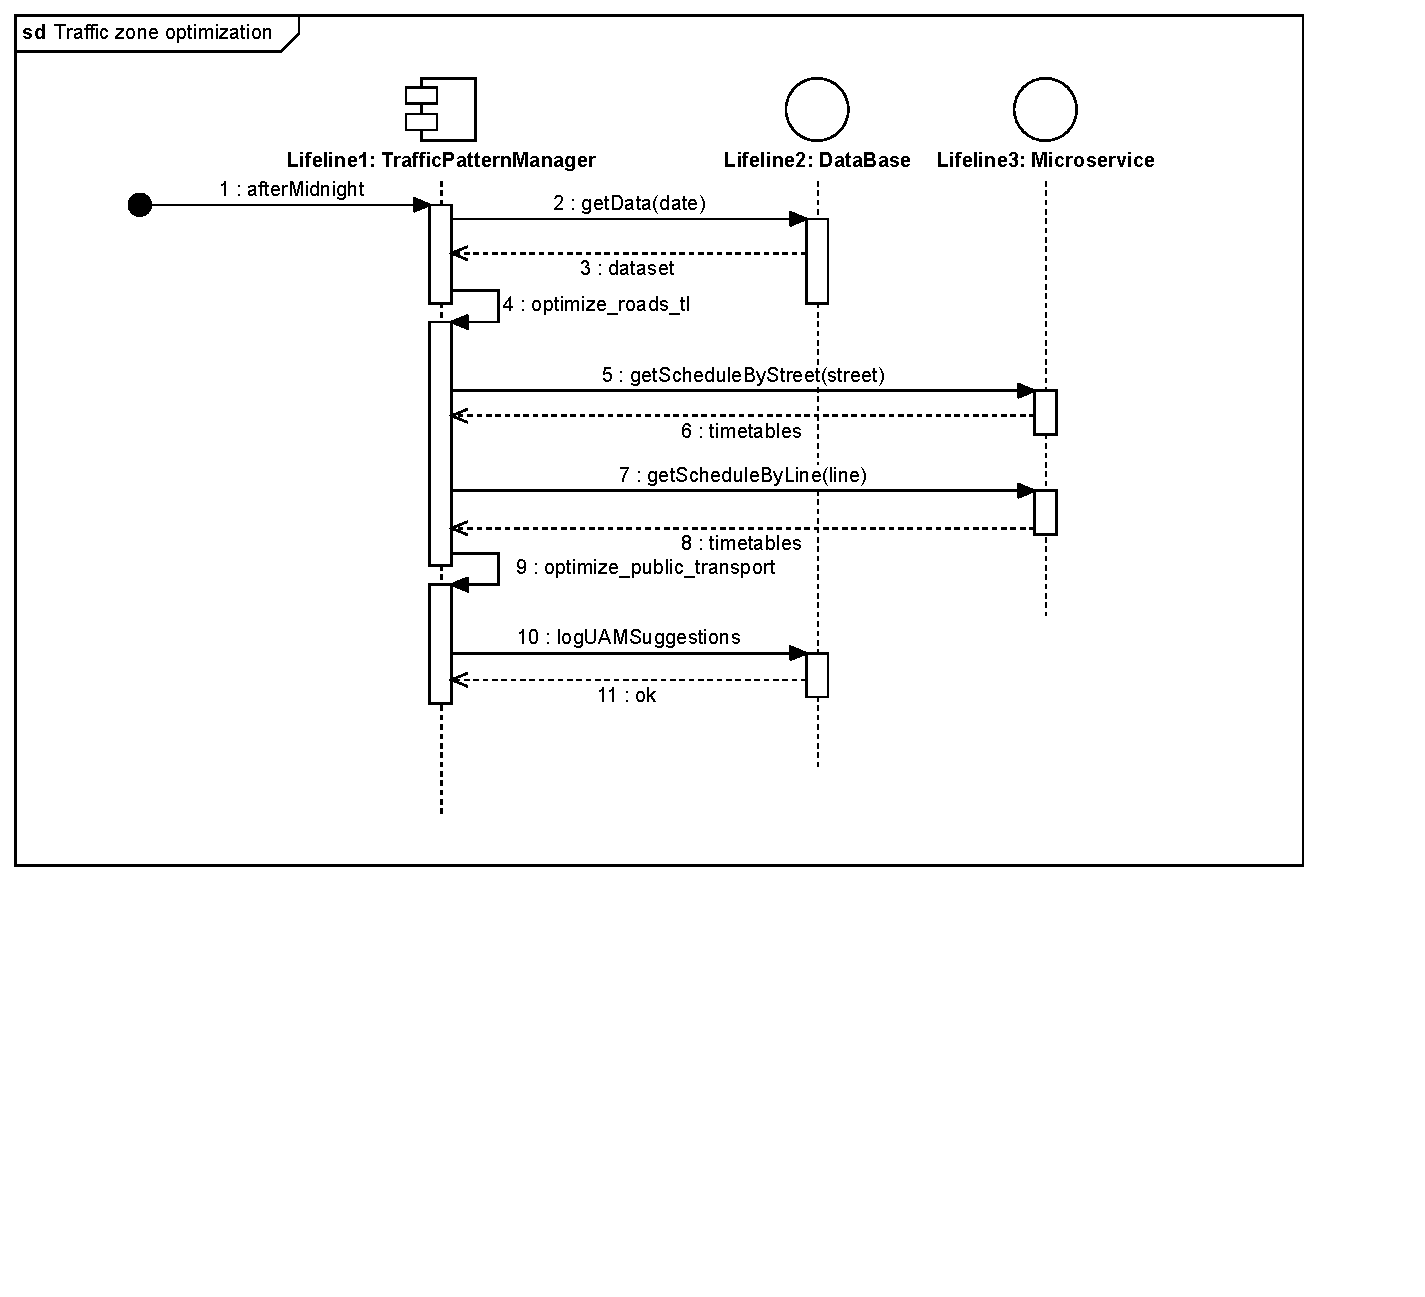
\includegraphics[width=\linewidth]{images/svg/traffic_zone_optimization.pdf}


This sequence diagram illustrates the data flow between TrafficPatternManager, database, and Microservice components for optimizing traffic zones, including both road traffic and public transportation optimization
\begin{enumerate}
  \item The process starts when the TrafficPatternManager receives an "afterMidnight" trigger or signal.
  \item TrafficPatternManager requests data from the database collected in the date passed as argument.
  \item The database responds by returning the data to the TrafficPatternManager.
  \item TrafficPatternManager analyzes the data to identify traffic patterns.
  \item TrafficPatternManager stores the patterns into the database.
  \item TrafficPatternManager tries to optimize the road traffic lights to reduce the traffic loads.
  \item	TrafficPatternManager asks for the timetables of the streets to the microsystem provided by the state.
  \item	The microsystem returns the street timetables.
  \item	TrafficPatternManager asks also for the timetables of the lines to the microsystem.
  \item	The microsystem returns the line timetables.
  \item TrafficPatternManager tries to optimize public transportation schedules.
  \item TrafficPatternManager logs the suggestions and stores the, into the database.
  \item The Microservice responds with an "ok" confirmation message, completing the sequence.
\end{enumerate}

\subsubsection{Event-specific Configuration}


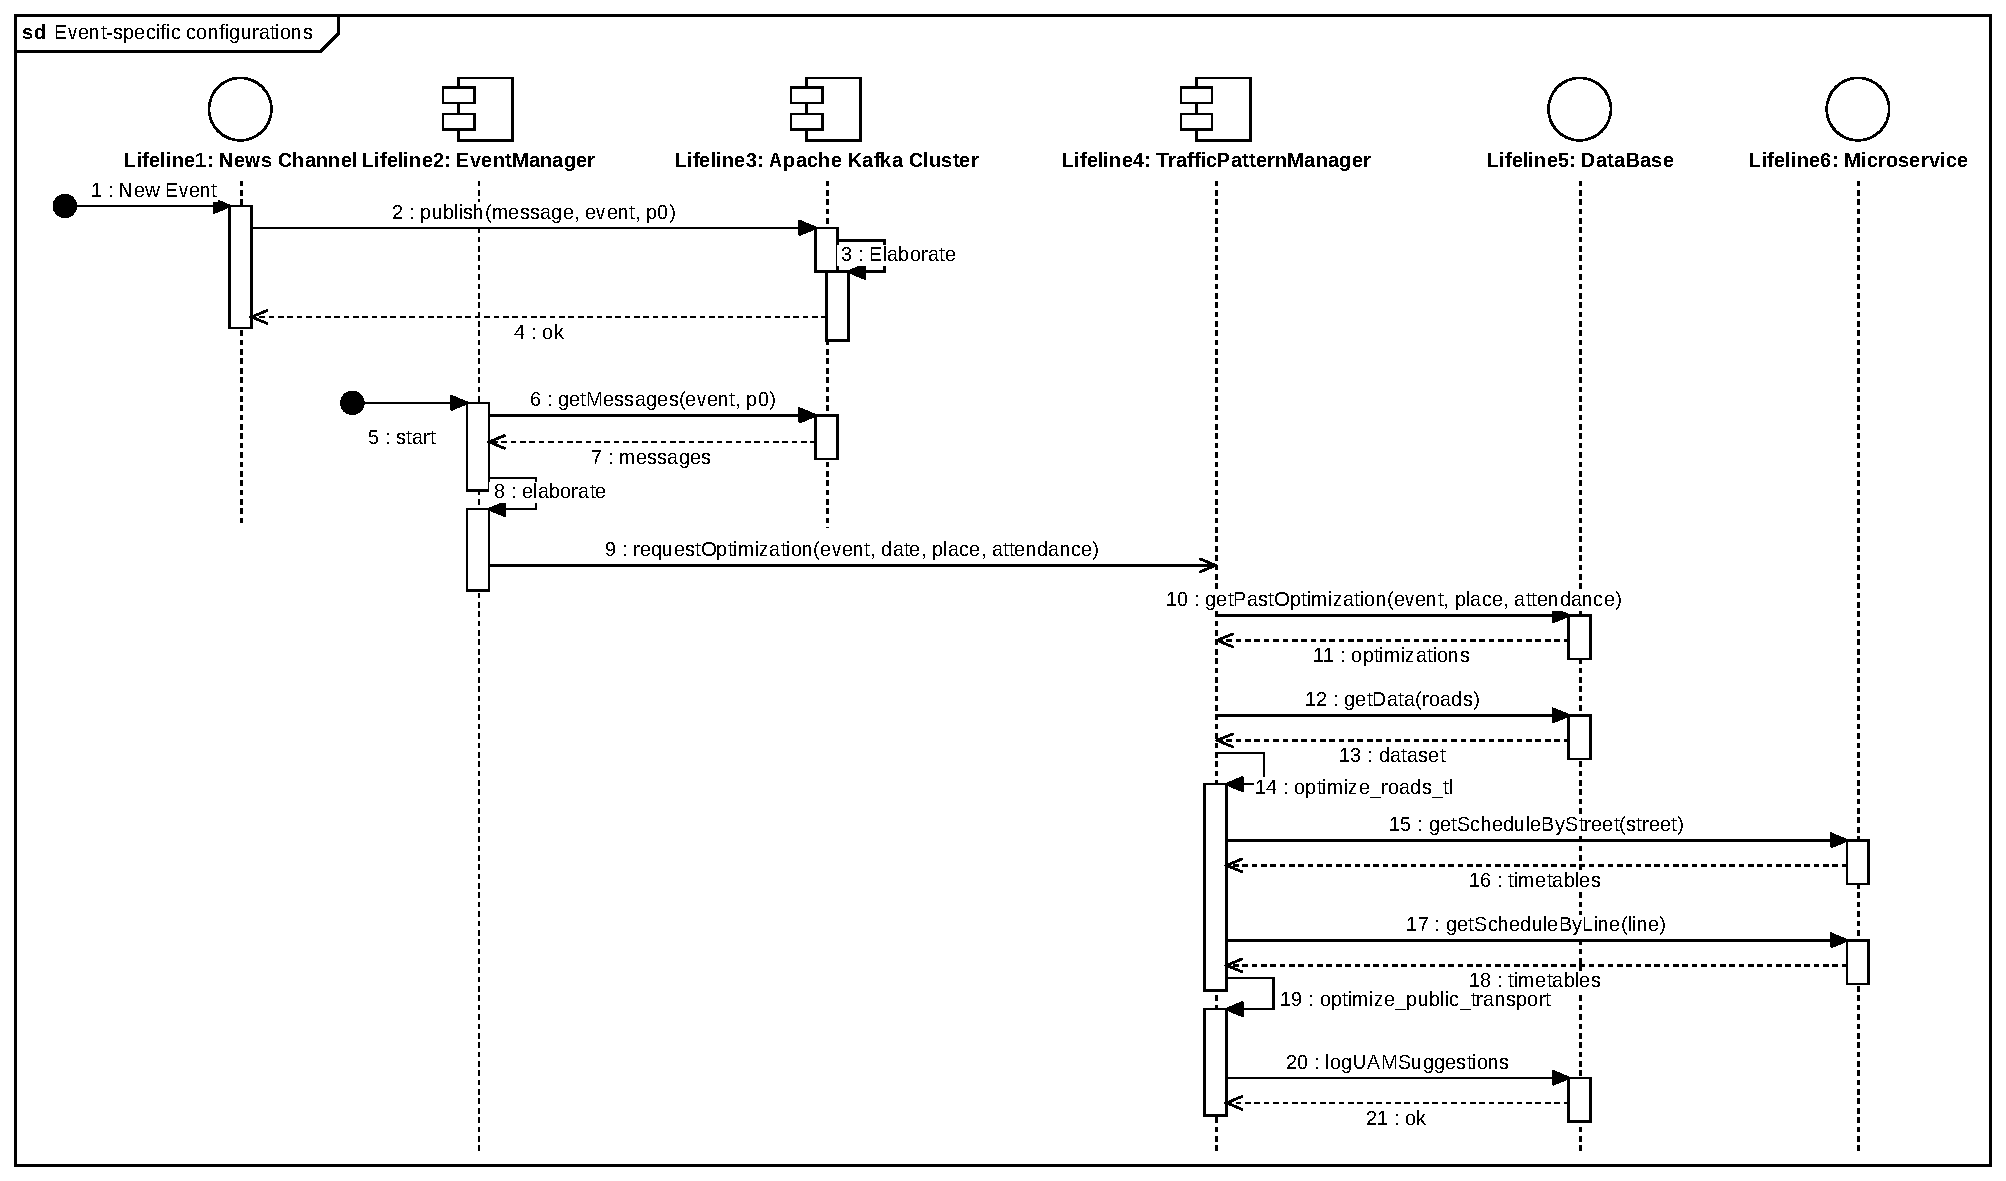
\includegraphics[width=\linewidth]{images/svg/event-specific_configurations.pdf}

This sequence diagram shows the communication and data flow involved in
adjusting traffic light timings based on crossing data.
\begin{enumerate}
  \item Ten minutes past midnight, an automatic process is started in the system and it is managed by the Traffic Pattern Manager.
  \item The Traffic Pattern Manager retrieves data from the DB by passing the current date.
  \item	The DB then returns a dataset to the Traffic Pattern Manager.
  \item	The TPM then optimizes the traffic flow for the whole system of traffic lights.
  \item	Then the TPM asks for the timetables of the streets to the microsystem provided by the state.
  \item	The microsystem returns the street timetables.
  \item	The TPM asks also for the timetables of the lines to the microsystem.
  \item	The microsystem returns the line timetables.
  \item	Then the system proceeds to optimize the public transport tables.
  \item	In the end the TPM logs the suggestions into the database.
  \item	The DB returns an ack message in case of successful write.
\end{enumerate}


\subsubsection{Citizen views public reports}


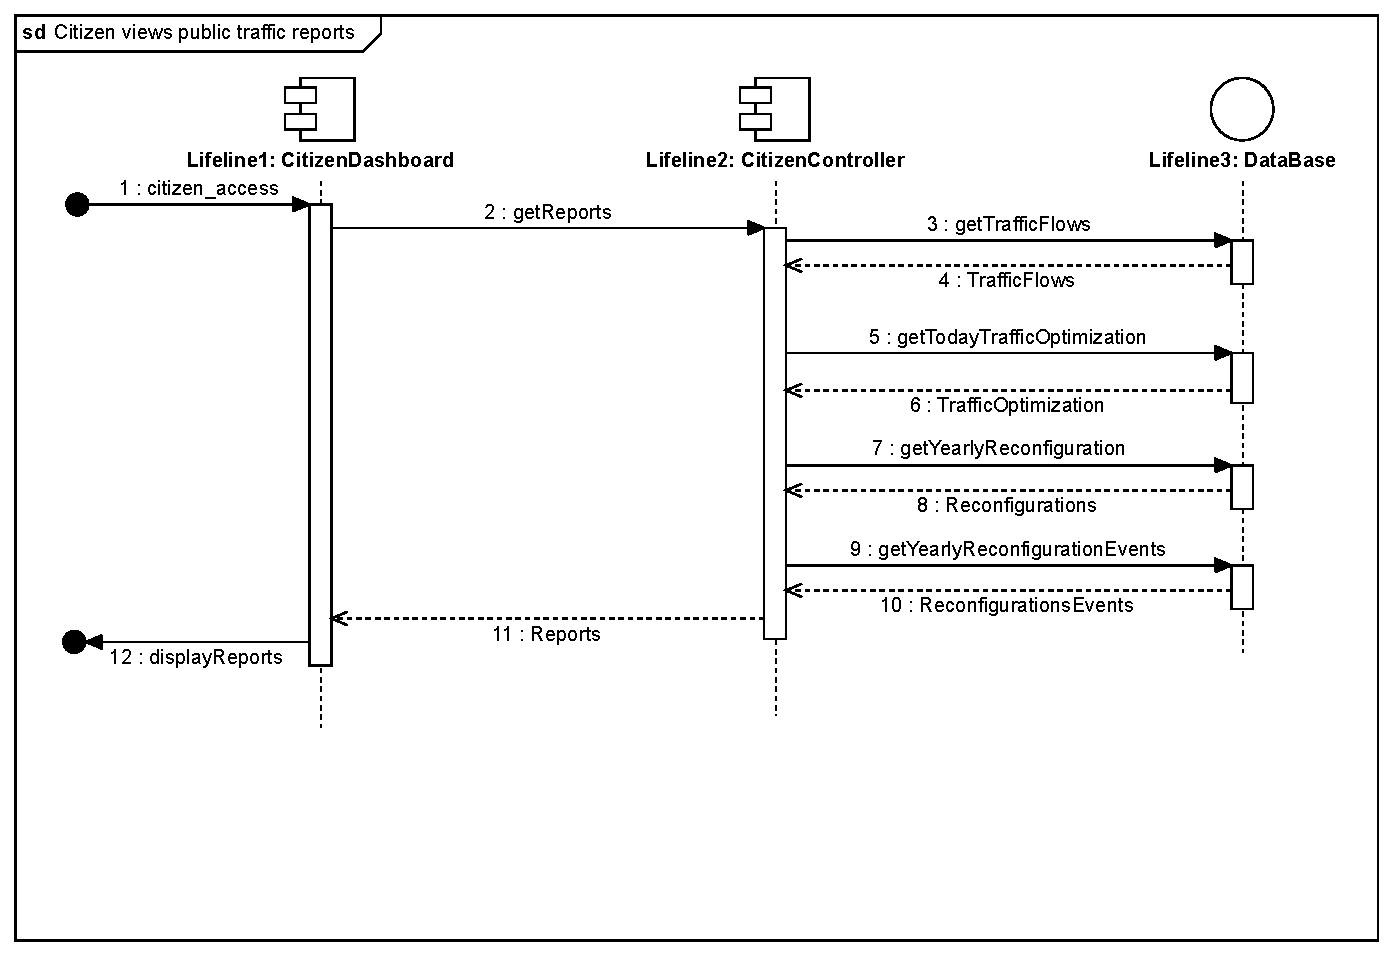
\includegraphics[width=\linewidth]{images/svg/citizen_views_public_traffic_reports.pdf}

This sequence diagram shows the communication and data flow involved in
adjusting traffic light timings based on crossing data.


\subsubsection{UAM configuration}

\includegraphics[width=\linewidth]{images/svg/uam_configuration.pdf}

This sequence diagram shows the communication and data flow involved in
adjusting traffic light timings based on crossing data.


\section{Critical points and design decisions}

\end{document}